
\de{ĐỀ THI HỌC KỲ II NĂM HỌC 2022-2023}{THPT Hướng Hoá - Quảng Trị}
\begin{center}
	\textbf{PHẦN 1 - TRẮC NGHIỆM}
\end{center}
\Opensolutionfile{ans}[ans/ans]
%Câu 1...........................
%
\begin{ex}%[0X2Y1-2]%[Dự án đề kiểm tra HKII NH22-23- TheHung Nguyebn]%[THPT Hướng Hóa - Quảng Trị]
 Có bao nhiêu cách sắp xếp $6$ học sinh theo một hàng dọc? 
	\choice
	{$5!$}
	{$6$}
	{$1$}
	{\True $6!$}
	\loigiai{Số cách xếp $6$ học sinh theo một hàng dọc là $6!$.
	}
\end{ex}

%2
\begin{ex}%[0H4Y3-2] %[Dự án đề kiểm tra HKII NH22-23- TheHung Nguyebn]%[THPT Hướng Hóa - Quảng Trị]
Trong các phương trình sau, phương trình nào là phương trình chính tắc của elip? 
	\choice
	{\True $\dfrac{x^2}{4}+\dfrac{y^2}{3}=1$}
	{$\dfrac{x^2}{4}-\dfrac{y^2}{3}=1$}
	{$\dfrac{x^2}{3}+\dfrac{y^2}{4}=1$}
	{$\dfrac{x}{4}+\dfrac{y}{3}=1$}
	\loigiai{Phương trình chính tắc của elip có dạng $\dfrac{x^2}{a^2}+\dfrac{y^2}{b^2}=1$ với $(a, b>0)$.\\
		Do đó phương trình $\dfrac{x^2}{4}+\dfrac{y^2}{3}=1$ thỏa đề bài.
	}
\end{ex}

%3
\begin{ex}%[0D4Y1-1]%[Dự án đề kiểm tra HKII NH22-23- TheHung Nguyebn]%[THPT Hướng Hóa - Quảng Trị]
Trong các biểu thức sau, biểu thức nào là tam thức bậc hai?
	\choice
	{$f(x)=(m-1)x^2+2 x+5$}
	{$f(x)=\dfrac{x^2+1}{x-2}$}
	{$f(x)=x+3$}
	{\True $f(x)=2x^2+x-5$}
	\loigiai{Tam thức bậc hai có dạng $f(x)=ax^2+bx+c$ với $a\ne 0$.\\
		Do đó $f(x)=2x^2+x-5$ thỏa đề bài.
	}
\end{ex}

%4
\begin{ex}%[0X2Y1-1]%[Dự án đề kiểm tra HKII NH22-23- TheHung Nguyebn]%[THPT Hướng Hóa - Quảng Trị]
Trong một tổ có $5$ bạn nam, $4$ bạn nữ. Hỏi có bao nhiêu cách chọn một bạn để phân công lao động? 
	\choice
	{$4$}
	{\True $9$}
	{$5$}
	{$20$}
	\loigiai{Có tổng cộng $9$ bạn, nên có $9$ cách chọn một bạn để phân công lao động.
	}
\end{ex}

%5
\begin{ex}%[0D3B2-3]%[Dự án đề kiểm tra HKII NH22-23- TheHung Nguyebn]%[THPT Hướng Hóa - Quảng Trị]
Cho parabol $(P)\colon y=x^2-2x-3$. Điểm nào sau đây là đỉnh của $(P)$? 
	\choice
	{$I(-1 ; 4)$}
	{\True $I(1 ;-4)$}
	{$I(-1 ;-4)$}
	{$I(1 ; 4)$}
	\loigiai{Hoành độ đỉnh là $x=-\dfrac{b}{2a}=-\dfrac{-2}{a}=1$.\\
		Với $x=1$, ta có $y=1-2-3=-4$.\\
		Tọa độ đỉnh $I(1 ;-4)$.
	}
\end{ex}

%6
\begin{ex}%[0X2B3-2]%[Dự án đề kiểm tra HKII NH22-23- TheHung Nguyebn]%[THPT Hướng Hóa - Quảng Trị]
Hệ số của $x^3$ trong khai triển $(1+x)^4$ là 
	\choice
	{\True $\mathrm{C}_4^3$}
	{$\mathrm{C}_4^2 x^2$}
	{$\mathrm{C}_4^3 x^2$}
	{$\mathrm{C}_4^2$}
	\loigiai{Ta có $(1+x)^4=\mathrm{C}_4^0\cdot1^4+ \mathrm{C}_4^1\cdot1^3\cdot x+\mathrm{C}_4^2\cdot 1^2\cdot x^2+\mathrm{C}_4^3\cdot 1\cdot x^3+\mathrm{C}_4^4x^4=1+4x+6x^2+4x^3+x^4$.
		Vậy hệ số của $x^3$ là $4$.
	}
\end{ex}

%7
\begin{ex}%[0X3B1-2]%[Dự án đề kiểm tra HKII NH22-23- TheHung Nguyebn]%[THPT Hướng Hóa - Quảng Trị]
Rút ra một lá bài từ bộ bài $52$ lá. Số phần tử của không gian mẫu là
	\choice
	{$\dfrac{1}{52}$}
	{$\dfrac{1}{4}$}
	{\True $52$}
	{$1$}
	\loigiai{Có $52$ cách rút ra $1$ lá bài, nên số phần tử của không gian mẫu là  $n(\Omega)=52$.
	}
\end{ex}

%8
\begin{ex}%[0X3B2-9]%[Dự án đề kiểm tra HKII NH22-23- TheHung Nguyebn]%[THPT Hướng Hóa - Quảng Trị]
Cho $A$ và $\overline{A}$ là hai biến cố đối nhau. Chọn khẳng định \textbf{đúng}.
	\choice
	{$\mathrm{P}(A)+\mathrm{P}(\overline{A})=0$}
	{\True $\mathrm{P}(A)+\mathrm{P}(\overline{A})=1$}
	{$\mathrm{P}(A)=1+\mathrm{P}(\overline{A})$}
	{$\mathrm{P}(A)=\mathrm{P}(\overline{A})$}
	\loigiai{Nếu $A$ và $\overline{A}$ là hai biến cố đối nhau thì $\mathrm{P}(A)+\mathrm{P}(\overline{A})=1$.
	}
\end{ex}

%9
\begin{ex}%[0H4Y2-2]%[Dự án đề kiểm tra HKII NH22-23- TheHung Nguyebn]%[THPT Hướng Hóa - Quảng Trị]
Trong mặt phẳng tọa độ $Oxy$, tìm phương trình của đường tròn có tâm $I(-3 ; 2)$ và bán kính $R=2$.
	\choice
	{$(x-3)^2+(y+2)^2=5$}
	{\True $(x+3)^2+(y-2)^2=4$}
	{$(x+3)^2+(y-2)^2=2$}
	{$(x-3)^2+(y+2)^2=4$}
	\loigiai{Phương trình của đường tròn có tâm $I(-3 ; 2)$ và bán kính $R=2$ là $(x+3)^2+(y-2)^2=4$.
	}
\end{ex}

%10
\begin{ex}%[0H4Y1-2]%[Dự án đề kiểm tra HKII NH22-23- TheHung Nguyebn]%[THPT Hướng Hóa - Quảng Trị]
Trong mặt phẳng $O x y$, tìm phương trình đường thẳng đi qua điểm $M(2 ; 0)$ và có một véc-tơ pháp tuyến $\vec{n}=(1 ;-2)$. 
	\choice
	{$x+2 y-2=0$}
	{\True $x-2 y-2=0$}
	{$x-2 y+2=0$}
	{$2 x+y-4=0$}
	\loigiai{Phương trình đường thẳng đi qua điểm $M(2; 0)$ và có một véc-tơ pháp tuyến $\overrightarrow{n}=(1 ;-2)$ là
		$$1\cdot(x-2)-2\cdot(y-0)=0\Leftrightarrow x-2y-2=0.$$
	}
\end{ex}

%11
\begin{ex}%[0X2B2-4]%[Dự án đề kiểm tra HKII NH22-23- TheHung Nguyebn]%[THPT Hướng Hóa - Quảng Trị]
Trong mặt phẳng cho $6$ điểm phân biệt trong đó không có $3$ điểm nào thẳng hàng. Số tam giác có đỉnh là $3$ trong số $6$ điểm đã cho là
	\choice
	{\True $\mathrm{C}_6^3$}
	{$6^3$}
	{$6!$}
	{$\mathrm{A}_6^3$}
	\loigiai{ Số tam giác có đỉnh là $3$ trong số $6$ điểm đã cho là $\mathrm{C}_6^3$.
	}
\end{ex}

%12
\begin{ex}%[0X3B2-3]%[Dự án đề kiểm tra HKII NH22-23- TheHung Nguyebn]%[THPT Hướng Hóa - Quảng Trị]
Một tổ học sinh gồm có $6$ nam và $4$ nữ. Chọn ngẫu nhiên $3$ học sinh. Xác suất sao cho $3$ học sinh được chọn có ít nhất $1$ học sinh nữ là
	\choice
	{$\dfrac{1}{30}$}
	{\True $\dfrac{5}{6}$}
	{$\dfrac{1}{6}$}
	{$\dfrac{1}{2}$}
	\loigiai{		
	Chọn ngẫu nhiên $3$ em trong $10$ học sinh có $\mathrm{C}_{10}^3=120$ cách.\\
	Suy ra số phần tử của không gian mẫu là $n(\Omega)=120$.\\
	Gọi $X$ là biến cố \lq\lq $3$ em được chọn có ít nhất $1$ nữ \rq\rq.\\
 Khi đó ta có biến cố đối $\overline{X}$: \lq\lq $3$ em được chọn không có em nữ nào\rq\rq.\\
	Suy ra $n({\overline{X}})=\mathrm{C}_6^3=20 \Rightarrow \mathrm P(\overline{X})=\dfrac{20}{120}=\dfrac{1}{6}$.\\
	Vậy $\mathrm P\mathrm(X)=1-\mathrm P(\overline{X})=1-\dfrac{1}{6}=\dfrac{5}{6}$	
	}
\end{ex}

%13
\begin{ex}%[0X3B2-1]%[Dự án đề kiểm tra HKII NH22-23- TheHung Nguyebn]%[THPT Hướng Hóa - Quảng Trị]
 Gieo một con súc sắc cân đối và đồng chất, xác suất để mặt có số chấm chẵn xuất hiện là
 	\choice
	{\True $\dfrac{1}{2}$}
	{$\dfrac{2}{3}$}
	{$\dfrac{1}{3}$}
	{$1$}
	\loigiai{Số phần tử không gian mẫu $n(\Omega)=6$.\\
		Gọi biến cố $\mathrm{A}$ \lq\lq mặt chẵn chấm xuất hiện\rq\rq.\\
		Ta có $A=\{2 ; 4 ; 6\} \Rightarrow n(A)=3$.
		Vậy xác suất $\mathrm P(A)=\dfrac{3}{6}=\dfrac{1}{2}$.
	}
\end{ex}

%14
\begin{ex}%[0X2B1-2]%[Dự án đề kiểm tra HKII NH22-23- TheHung Nguyebn]%[THPT Hướng Hóa - Quảng Trị]
Một câu lạc bộ có $20$ thành viên. Tính số cách chọn một ban quản lí gồm $1$ chủ tịch, $1$ phó chủ tịch và $1$ thư kí.
	\choice
	{$1\,140$}
	{\True $6\,840$}
	{ $13\,800$}
	{$6\,900$}
	\loigiai{Số cách chọn một ban quản lí gồm $1$ chủ tịch, $1$ phó chủ tịch và $1$ thư kí là $20\cdot 19\cdot 18=6840$ cách.
	}
\end{ex}

%15
\begin{ex}%[0D4B1-3]%[Dự án đề kiểm tra HKII NH22-23- TheHung Nguyebn]%[THPT Hướng Hóa - Quảng Trị]
\immini{Cho hàm số bậc hai $f(x)=ax^2+b x+c$ với $ (a \neq 0)$ có đồ thị như hình vẽ.
	Chọn khẳng định \textbf{đúng}.	
	\choice
	{\True $f(x)>0, \forall x \in(-\infty ; 1) \cup(4 ;+\infty)$}
	{$f(x)<0, \forall x \in(0 ; 4)$}
	{$f(x)<0, \forall x \in(-1 ; 4)$}
	{$f(x)>0, \forall x \in(3 ;+\infty)$}}{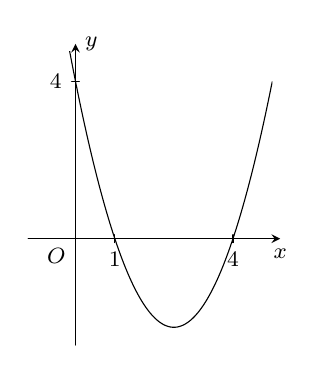
\begin{tikzpicture}[scale=.5, font=\footnotesize, line join=round, line cap=round, >=stealth]
		\def\xmin{-1}\def\xmax{5}\def\ymin{-2.5}\def\ymax{4.75}
		\draw[->] (\xmin-0.2,0)--(\xmax+0.2,0) node[below] {\footnotesize $x$};
		\draw[->] (0,\ymin-0.2)--(0,\ymax+0.2) node[right] {\footnotesize $y$};
		\draw (0,0) node [below left] {\footnotesize $O$};
		\foreach \x in {1,4}\draw (\x,0.1)--(\x,-0.1) node [below] {\footnotesize $\x$};
		\foreach \y in {4}\draw (0.1,\y)--(-0.1,\y) node [left] {\footnotesize $\y$};
		\clip (\xmin,\ymin) rectangle (\xmax,\ymax);
		\draw[smooth,samples=200,domain=\xmin:\xmax] plot (\x,{1*((\x)^2)+-5*\x+4});
\end{tikzpicture}} 
	\loigiai{Dựa vào đồ thị ta có $f(x)>0, \forall x \in(-\infty ; 1) \cup(4 ;+\infty)$.
	}
\end{ex}

%16
\begin{ex}%[0X3B2-3]%[Dự án đề kiểm tra HKII NH22-23- TheHung Nguyebn]%[THPT Hướng Hóa - Quảng Trị]
Một tổ có $7$ nam và $3$ nữ. Chọn ngẫu nhiên $2$ người. Xác suất sao cho $2$ người được chọn đều là nữ là
	\choice
	{$\dfrac{7}{15}$}
	{$\dfrac{8}{15}$}
	{$\dfrac{2}{15}$}
	{\True $\dfrac{1}{15}$}
	\loigiai{Chọn ngẫu nhiên $2$ người có $n(\Omega)=\mathrm{C}_{10}^2$ cách.\\
		Gọi $A$ là biến cố  \lq\lq $2$ người được chọn đều là nữ. \rq\rq\\
		 Ta có $n(A)=\mathrm{C}_3^2$.
		Do đó sác xuất cần tìm là
		$\mathrm{P}(A)=\dfrac{\mathrm{C}_3^2}{\mathrm{C}_{10}^2}=\dfrac{1}{15}$.
	}
\end{ex}

%17
\begin{ex}%[0X3B2-3]%[Dự án đề kiểm tra HKII NH22-23- TheHung Nguyebn]%[THPT Hướng Hóa - Quảng Trị]
Khai triển $(x-1)^5$ bằng
	\choice
	{\True $x^5-5 x^4+10 x^3-10 x^2+5 x-1$}
	{$x^5+5 x^4+10 x^3+10 x^2+5 x+1$}
	{$x^5-5 x^4-10 x^3-10 x^2-5 x-1$}
	{$x^5+5 x^4-10 x^3+10 x^2-5 x+1$}
	\loigiai{Ta có
	
		\begin{eqnarray*}
			(x-1)^5&=&[x+(-1)]^5\\
			&=&\mathrm{C}_5^0\cdot x^5+\mathrm{C}_5^1\cdot x^4\cdot (-1)+\mathrm{C}_5^2\cdot x^3\cdot (-1)^2+\mathrm{C}_5^3\cdot x^2\cdot (-1)^3+\mathrm{C}_5^4\cdot x^1\cdot (-1)^4+\mathrm{C}_5^5\cdot (-1)^5\\
			&=& x^5+5x^4(-1)+10x^3(-1)^2+10x^2(-1)^3+5x(-1)^4+(-1)^5\\
			&=&x^5-5x^4+10x^3-10x^2+5x-1.
		\end{eqnarray*}
	}
\end{ex}

%18
\begin{ex}%[0X2B1-5]%[Dự án đề kiểm tra HKII NH22-23- TheHung Nguyebn]%[THPT Hướng Hóa - Quảng Trị]
Cho $6$ chữ số $1,2,3,4,5,6$. Có bao nhiêu số tự nhiên có $4$ chữ số khác nhau được lập từ $6$ chữ số đó? 
	\choice
	{$256$}
	{\True $360$}
	{$125$}
	{$60$}
	\loigiai{Số số tự nhiên có $4$ chữ số khác nhau được lập từ $6$ chữ số trên thỏa đề bài là $\mathrm{A}_6^4=360$ số.
	}
\end{ex}

%19
\begin{ex}% [0H4B1-2]%[Dự án đề kiểm tra HKII NH22-23- TheHung Nguyebn]%[THPT Hướng Hóa - Quảng Trị]
Trong mặt phẳng $Oxy$, phương trình tham số của đường thẳng $\Delta$ đi qua điểm $A(-4 ; 2)$ nhận $\vec{u}=(-2 ; 3)$ làm véc-tơ chỉ phương là
	\choice
	{\True $\heva{&x=-4-2t\\ &y=2+3t}$}
	{$\heva{&x=4+2t\\ &y=-2-3t}$}
	{$\heva{&x=-2-4t\\ &y=3+2t}$}
	{$\heva{&x=-2-2t\\ &y=-1+3t}$}
	\loigiai{Phương trình tham số của đường thẳng $\Delta$ đi qua điểm $A(-4 ; 2)$ nhận $\vec{u}=(-2 ; 3)$ làm véc-tơ chỉ phương là $\heva{&x=-4-2t\\ &y=2+3t.}$
	}
\end{ex}

%20
\begin{ex}%[0D4B3-1]%[Dự án đề kiểm tra HKII NH22-23- TheHung Nguyebn]%[THPT Hướng Hóa - Quảng Trị]
Nghiệm của phương trình $\sqrt{2 x^2-5 x-9}=\sqrt{x^2-3}$ thuộc khoảng nào sau đây? 
	\choice
	{\True $(5 ; 7)$}
	{$(2 ; 4)$}
	{$(3 ; 5)$}
	{$(1 ; 3)$}
	\loigiai{Ta có \begin{eqnarray*}
			& & \sqrt{2 x^2-5 x-9}=\sqrt{x^2-3}\\
			&\Rightarrow & 2x^2-5x-9=x^2-3\\
			&\Rightarrow & x^2-5x-6=0\\
			&\Rightarrow & \hoac{& x=-1 \\ & x=6.}
		\end{eqnarray*}
	Thử lại thì $x=6$ là nghiệm của phương trình.
	}
\end{ex}


\Closesolutionfile{ans}
%\begin{center}
%	\textbf{ĐÁP ÁN}
%	\inputansbox{10}{ans/ans}	
%\end{center}
\begin{center}
	\textbf{PHẦN 2 - TỰ LUẬN}
\end{center}

\begin{bt}%[0H4B1-3]%[Dự án đề kiểm tra HKII NH22-23- TheHung Nguyebn]%[THPT Hướng Hóa - Quảng Trị]
	Xét vị trí tương đối của hai đường thẳng 
	$d_1\colon\heva{&x=-2+t\\ &y=3-2t}$ và $d_2\colon\heva{&x=3-2t'\\ &y=-1+4t'.}$
	\loigiai{
	Ta có $d_1$ có véc-tơ chỉ phương $\overrightarrow{u_1}(1 ;-2)$ và $d_2$ có véc-tơ chỉ phương $\overrightarrow{u_2}(-2 ; 4)$.\\ Suy ra $\overrightarrow{u_2}=-2\overrightarrow{u_1}$ nên $\overrightarrow{u_1},\overrightarrow{u_2}$ cùng phương. Do đó, chúng song song hoặc trùng nhau.\\
	Mặt khác $M(-2 ; 3)\in d_1$ nhưng $M\notin d_2$ nên $d_1\parallel d_2$.	
}
	
\end{bt}

\begin{bt}%[0X3B2-3]%[Dự án đề kiểm tra HKII NH22-23- TheHung Nguyebn]%[THPT Hướng Hóa - Quảng Trị]
	Trong một cuộc tổng điều tra dân số, điều tra viên chọn ngẫu nhiên một gia đình có ba người con và quan tâm giới tính của ba người con này.
	\begin{enumerate}
		\item  Vẽ sơ đồ hình cây để mô tả các phần tử của không gian mẫu.
		\item Giả thiết rằng khả năng sinh con trai và khả năng sinh con gái là như nhau. Tính xác suất để gia đình đó có một con gái và hai con trai.
	\end{enumerate}
\loigiai{
	\begin{enumerate}
	\item  Ký hiệu $T\colon$ Con trai, $G\colon$ Con gái.
	\begin{center}
		\begin{tikzpicture}
			\tikzstyle{level 1}=[sibling distance=50mm]
			\tikzstyle{level 2}=[sibling distance=20mm]
			\tikzstyle{level 3}=[sibling distance=10mm]
			\tikzstyle{level 4}=[sibling distance=10mm]
			\node at (-6,-1.5){Con thứ $1$};
			\node at (-6,-2.92){Con thứ $2$};
			\node at (-6,-4.42){Con thứ $3$};
			\node{ }
			child
			{
				node{T}
				child
				{
					node{T}
					child{node{T}}
					child{node{G}}
				}
				child
				{
					node{G}
					child{node{T}}
					child{node{G}}
				}
			}
			child
			{
				node{G}
				child
				{
					node{T}
					child{node{T}}
					child{node{G}}
				}            
				child
				{
					node{G}
					child{node{T}}
					child{node{G}}
				}
			};    
			
		\end{tikzpicture}
	\end{center}
	
	
	Sơ đồ cây có không gian mẫu là
	$$
	\Omega=\{\text { TTT ; TTG ; TGT ; TGG ; GTT; GTG; GGT; GGG }\}.
	$$
	\item  Giả thiết rằng khả năng sinh con trai và khả năng sinh con gái là như nhau. Tính xác suất để gia đình đó có một con gái và hai con trai.\\
	Ta có $n(\Omega)=8$.
	Biến cố $A$ \lq\lq gia đình đó có một con gái và hai con trai \rq\rq.\\
	Nên $A=\{TTG, TGT, GTT \}$ suy ra $n(A)=3$.\\
	Từ đó $\mathrm{P}(A)=\dfrac{n(A)}{n(\Omega)}=\dfrac{3}{8}$.
\end{enumerate}
}
\end{bt}


\begin{bt}%[0X2B3-2]%[Dự án đề kiểm tra HKII NH22-23- TheHung Nguyebn]%[THPT Hướng Hóa - Quảng Trị]
	Xác định hạng tử không chứa $x$ trong khai triển của $\left(x^3-\dfrac{2}{x}\right)^4$.
	\loigiai{Ta có 
		\begin{eqnarray*}
			\left(x^3-\dfrac 2 x\right)^4&=&\mathrm{C}_4^0\left(x^3\right)^4+\mathrm{C}_4^1\left(x^3\right)^3\left(-\dfrac 2 x\right)+\mathrm{C}_4^2\left(x^3\right)^2\left(-\dfrac 2 x\right)^2+\mathrm{C}_4^3x^3\left(-\dfrac 2 x\right)^3+\mathrm{C}_4^4\left(-\dfrac 2 x\right)^4\\
			&=& x^{12}-8x^8+24x^4-32+\dfrac{16}{x^4}.	
		\end{eqnarray*}
	Vậy hạng tử không chứa $x$ là $-32$. 
	}
\end{bt}


\begin{bt}%[0X3K2-3]%[Dự án đề kiểm tra HKII NH22-23- TheHung Nguyebn]%[THPT Hướng Hóa - Quảng Trị]
	Trường THPT Hướng Hóa có $28$ lớp, trong đó khối $10$ có $10$ lớp, khối $11$ có $9$ lớp, khối $12$ có $9$ lớp, mỗi lớp có một học sinh làm bí thư. Ban chấp hành Đoàn trường chọn ngẫu nhiên $15$ em bí thư tham gia một cuộc khảo sát về tình hình an ninh trật tự trong nhà trường. Tính xác suất để $15$ em được chọn có đủ cả ba khối?
	\loigiai{
	Số phần tử của không gian mẫu là $n(\Omega)=\mathrm{C}_{28}^{15}$.\\
	Gọi biến cố $A\colon$ \lq\lq $15$ em được chọn có đủ cả ba khối\rq\rq.\\
	Suy ra biến cố đối $\overline{A}\colon$ \lq\lq $15$ em được chọn không đủ cả ba khối\rq\rq.\\
	Vì mỗi khối số bí thư đều nhỏ hơn $15$ nên xảy ra các phương án sau:
	\begin{enumerate}[•]
		\item	Phương án 1: Chỉ có học sinh ở khối $10$ và $11$ nên có $\mathrm{C}_{19}^{15}$ cách.
	\item	Phương án $2\colon$ Chỉ có học sinh ở khối $10$ và $12$ nên có $\mathrm{C}_{19}^{15}$ cách.
	\item	Phương án $3\colon$ Chỉ có học sinh ở khối $11$ và $12$ nên có $\mathrm{C}_{18}^{15}$ cách.
	\end{enumerate}	
	Khi đó, $n(\overline{A})=\mathrm{C}_{18}^{15}+\mathrm{C}_{19}^{15}+\mathrm{C}_{19}^{15}=8568$.\\
	Xác suất xảy ra của biến cố $A$ là $\mathrm{P}(A)=1-P(\overline{A})=1-\dfrac{8568}{C_{28}^{15}}=\dfrac{4369}{4370}$
}
\end{bt}

\begin{bt}%[0X3G2-8]%[Dự án đề kiểm tra HKII NH22-23- TheHung Nguyebn]%[THPT Hướng Hóa - Quảng Trị]
	Chọn ngẫu nhiên ba số phân biệt $a,b,c$ từ tập $S=\{1,2, \ldots ., 50\}$. Tính xác suất để $a^2+b^2+c^2$ chia hết cho $3$.
	\loigiai{Gọi biến cố $A$: \lq\lq Ba số $a, b, c$ phân biệt, chọn được từ tập $S$, sao cho $a^2+b^2+c^2$ chia hết cho $3$\rq\rq.\\
	Số phần tử của không gian mẫu $n(\Omega)=\mathrm{C}_{50}^3$.\\
	Ta có 
	\begin{itemize}
		\item	Nếu $n=3 k \Rightarrow n^2=9 k^2 \Rightarrow n^2$ chia hết cho $3$.
		\item Nếu $n=3 k+1 \Rightarrow n^2=9 k^2+6 k+1 \Rightarrow n^2$ chia cho $3$ có số dư là $1$.
		\item Nếu $n=3 k+2 \Rightarrow n^2=9 k^2+12 k+4 \Rightarrow n^2$ chia cho $3$ có số dư là $1$.
	\end{itemize}
	Do đó đế $a^2+b^2+c^2$ chia hết cho $3$ thì
	\begin{itemize}
		\item  Trường hợp $1\colon$ $a, b, c$ cùng chia hết cho $3$.
		\item Trường hợp $2\colon$ $a, b, c$ cùng không chia hết cho $3$.
	\end{itemize}
	Tập $S=\{1,2, \ldots, 50\}$ có $16$ phần tử chia hết cho $3$ và $34$ phần tử không chia hết cho $3$.\\
	Suy ra $n(A)=\mathrm{C}_{16}^3+C_{34}^3$.\\
Vậy 	$ \mathrm{P}(A)=\dfrac{n(A)}{n(\Omega)}=\dfrac{\mathrm{C}_{16}^3+\mathrm{C}_{34}^3}{\mathrm{C}_{50}^3}=\dfrac{409}{1225}$.

	}
\end{bt}